\documentclass[border=5pt]{standalone}
\usepackage{fontspec,unicode-math}
\setmainfont{Noto Serif}
\setmathfont{STIXTwoMath-Regular.otf}
\usepackage{tikz}
\usetikzlibrary{arrows.meta,calc,patterns,decorations.markings,decorations.pathmorphing}
\tikzset{lev/.style={line width=1.25pt,line cap=butt},
 fine/.style={line width=.60pt},band/.style={line width=.57pt},
 curve/.style={line width=1.35pt,line cap=round,line join=round},
 ax/.style={line width=.65pt,-{Latex[length=2.3mm,width=1.3mm]}},
 ray/.style={line width=.68pt,-{Latex[length=2.0mm,width=1.10mm]}},
 dimension/.style={line width=.57pt,{Latex[length=1.7mm,width=.9mm]}-{Latex[length=1.7mm,width=.9mm]}},
 flow/.style={line width=.68pt,postaction={decorate},decoration={markings,mark=at position .66 with {\arrow{Latex[length=2mm,width=1.1mm]}}}},
 lab/.style={font=\fontsize{13}{16}\selectfont,inner sep=1.3pt},
 small/.style={font=\fontsize{11}{13}\selectfont,inner sep=1.2pt},
 tinytext/.style={font=\fontsize{10}{12}\selectfont,inner sep=1pt},
 panel/.style={font=\fontsize{14}{16}\selectfont\itshape,inner sep=0pt}}
\pagestyle{empty}
\begin{document}
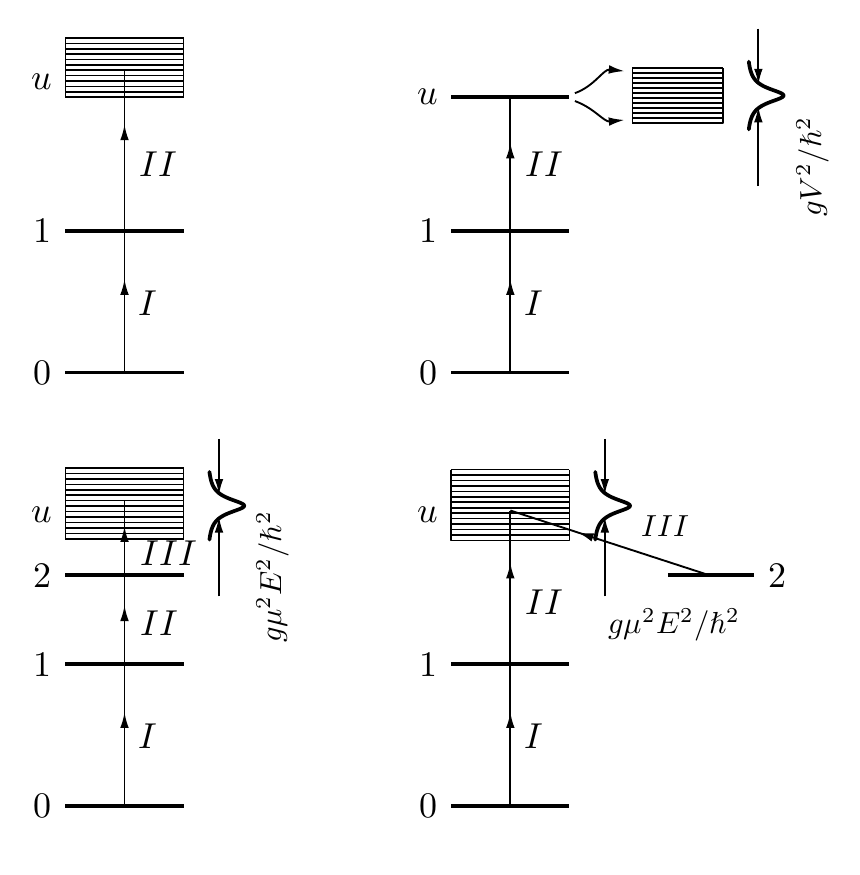
\begin{tikzpicture}[x=1cm,y=1cm,line join=round]
\begin{scope}[shift={(0,5.5)}]
\draw[lev] (0.5500,0.5500)--++(1.5000,0);
\node[lab,anchor=east] at (0.4300,0.5500) {$0$};
\draw[lev] (0.5500,2.3500)--++(1.5000,0);
\node[lab,anchor=east] at (0.4300,2.3500) {$1$};
\draw[flow] (1.3,.55)--(1.3,2.35);\node[lab,anchor=west] at (1.43,1.43) {$I$};
\draw[band] (0.5500,4.0500)--++(1.5000,0);
\draw[band] (0.5500,4.1182)--++(1.5000,0);
\draw[band] (0.5500,4.1864)--++(1.5000,0);
\draw[band] (0.5500,4.2545)--++(1.5000,0);
\draw[band] (0.5500,4.3227)--++(1.5000,0);
\draw[band] (0.5500,4.3909)--++(1.5000,0);
\draw[band] (0.5500,4.4591)--++(1.5000,0);
\draw[band] (0.5500,4.5273)--++(1.5000,0);
\draw[band] (0.5500,4.5955)--++(1.5000,0);
\draw[band] (0.5500,4.6636)--++(1.5000,0);
\draw[band] (0.5500,4.7318)--++(1.5000,0);
\draw[band] (0.5500,4.8000)--++(1.5000,0);
\draw[fine] (0.5500,4.8000)--(0.5500,4.0500)--++(1.5000,0)--++(0,0.7500);
\draw[flow] (1.3,2.35)--(1.3,4.4);\node[lab,anchor=west] at (1.44,3.2) {$II$};\node[lab,anchor=east] at (.43,4.25) {$u$};
\node[panel] at (1.3,.05) {а};
\end{scope}
\begin{scope}[shift={(4.9,5.5)}]
\draw[lev] (0.5500,0.5500)--++(1.5000,0);
\node[lab,anchor=east] at (0.4300,0.5500) {$0$};
\draw[lev] (0.5500,2.3500)--++(1.5000,0);
\node[lab,anchor=east] at (0.4300,2.3500) {$1$};
\draw[flow] (1.3,.55)--(1.3,2.35);\node[lab,anchor=west] at (1.43,1.43) {$I$};
\draw[lev] (0.5500,4.0500)--++(1.5000,0);
\node[lab,anchor=east] at (0.4300,4.0500) {$u$};
\draw[band] (2.8500,3.7200)--++(1.1500,0);
\draw[band] (2.8500,3.7836)--++(1.1500,0);
\draw[band] (2.8500,3.8473)--++(1.1500,0);
\draw[band] (2.8500,3.9109)--++(1.1500,0);
\draw[band] (2.8500,3.9745)--++(1.1500,0);
\draw[band] (2.8500,4.0382)--++(1.1500,0);
\draw[band] (2.8500,4.1018)--++(1.1500,0);
\draw[band] (2.8500,4.1655)--++(1.1500,0);
\draw[band] (2.8500,4.2291)--++(1.1500,0);
\draw[band] (2.8500,4.2927)--++(1.1500,0);
\draw[band] (2.8500,4.3564)--++(1.1500,0);
\draw[band] (2.8500,4.4200)--++(1.1500,0);
\draw[fine] (2.8500,4.4200)--(2.8500,3.7200)--++(1.1500,0)--++(0,0.7000);
\draw[flow] (1.3,2.35)--(1.3,4.05);\node[lab,anchor=west] at (1.44,3.2) {$II$};\draw[ray] (2.12,4.1) to[out=20,in=174] (2.75,4.38);\draw[ray] (2.12,4.0) to[out=-20,in=186] (2.75,3.76);
\draw[curve] (4.32887,3.64000)--(4.32973,3.64667)--(4.33062,3.65333)--(4.33156,3.66000)--(4.33254,3.66667)--(4.33356,3.67333)--(4.33463,3.68000)--(4.33576,3.68667)--(4.33693,3.69333)--(4.33817,3.70000)--(4.33946,3.70667)--(4.34082,3.71333)--(4.34225,3.72000)--(4.34375,3.72667)--(4.34533,3.73333)--(4.34700,3.74000)--(4.34876,3.74667)--(4.35061,3.75333)--(4.35256,3.76000)--(4.35462,3.76667)--(4.35681,3.77333)--(4.35912,3.78000)--(4.36156,3.78667)--(4.36416,3.79333)--(4.36691,3.80000)--(4.36983,3.80667)--(4.37293,3.81333)--(4.37623,3.82000)--(4.37975,3.82667)--(4.38350,3.83333)--(4.38749,3.84000)--(4.39176,3.84667)--(4.39632,3.85333)--(4.40119,3.86000)--(4.40641,3.86667)--(4.41200,3.87333)--(4.41799,3.88000)--(4.42441,3.88667)--(4.43131,3.89333)--(4.43871,3.90000)--(4.44666,3.90667)--(4.45519,3.91333)--(4.46436,3.92000)--(4.47421,3.92667)--(4.48478,3.93333)--(4.49610,3.94000)--(4.50823,3.94667)--(4.52119,3.95333)--(4.53500,3.96000)--(4.54967,3.96667)--(4.56520,3.97333)--(4.58153,3.98000)--(4.59862,3.98667)--(4.61633,3.99333)--(4.63453,4.00000)--(4.65299,4.00667)--(4.67143,4.01333)--(4.68952,4.02000)--(4.70686,4.02667)--(4.72300,4.03333)--(4.73746,4.04000)--(4.74976,4.04667)--(4.75945,4.05333)--(4.76615,4.06000)--(4.76957,4.06667)--(4.76957,4.07333)--(4.76615,4.08000)--(4.75945,4.08667)--(4.74976,4.09333)--(4.73746,4.10000)--(4.72300,4.10667)--(4.70686,4.11333)--(4.68952,4.12000)--(4.67143,4.12667)--(4.65299,4.13333)--(4.63453,4.14000)--(4.61633,4.14667)--(4.59862,4.15333)--(4.58153,4.16000)--(4.56520,4.16667)--(4.54967,4.17333)--(4.53500,4.18000)--(4.52119,4.18667)--(4.50823,4.19333)--(4.49610,4.20000)--(4.48478,4.20667)--(4.47421,4.21333)--(4.46436,4.22000)--(4.45519,4.22667)--(4.44666,4.23333)--(4.43871,4.24000)--(4.43131,4.24667)--(4.42441,4.25333)--(4.41799,4.26000)--(4.41200,4.26667)--(4.40641,4.27333)--(4.40119,4.28000)--(4.39632,4.28667)--(4.39176,4.29333)--(4.38749,4.30000)--(4.38350,4.30667)--(4.37975,4.31333)--(4.37623,4.32000)--(4.37293,4.32667)--(4.36983,4.33333)--(4.36691,4.34000)--(4.36416,4.34667)--(4.36156,4.35333)--(4.35912,4.36000)--(4.35681,4.36667)--(4.35462,4.37333)--(4.35256,4.38000)--(4.35061,4.38667)--(4.34876,4.39333)--(4.34700,4.40000)--(4.34533,4.40667)--(4.34375,4.41333)--(4.34225,4.42000)--(4.34082,4.42667)--(4.33946,4.43333)--(4.33817,4.44000)--(4.33693,4.44667)--(4.33576,4.45333)--(4.33463,4.46000)--(4.33356,4.46667)--(4.33254,4.47333)--(4.33156,4.48000)--(4.33062,4.48667)--(4.32973,4.49333)--(4.32887,4.50000);
\draw[ray] (4.45,4.92)--(4.45,4.21);\draw[ray] (4.45,2.9200000000000004)--(4.45,3.93);
\node[small,rotate=90,anchor=north] at (4.88,3.1700000000000004) {$gV^2/\hbar^2$};
\node[panel] at (1.3,.05) {б};
\end{scope}
\begin{scope}[shift={(0,0)}]
\draw[lev] (0.5500,0.5500)--++(1.5000,0);
\node[lab,anchor=east] at (0.4300,0.5500) {$0$};
\draw[lev] (0.5500,2.3500)--++(1.5000,0);
\node[lab,anchor=east] at (0.4300,2.3500) {$1$};
\draw[flow] (1.3,.55)--(1.3,2.35);\node[lab,anchor=west] at (1.43,1.43) {$I$};
\draw[lev] (0.5500,3.4800)--++(1.5000,0);
\node[lab,anchor=east] at (0.4300,3.4800) {$2$};
\draw[band] (0.5500,3.9400)--++(1.5000,0);
\draw[band] (0.5500,4.0092)--++(1.5000,0);
\draw[band] (0.5500,4.0785)--++(1.5000,0);
\draw[band] (0.5500,4.1477)--++(1.5000,0);
\draw[band] (0.5500,4.2169)--++(1.5000,0);
\draw[band] (0.5500,4.2862)--++(1.5000,0);
\draw[band] (0.5500,4.3554)--++(1.5000,0);
\draw[band] (0.5500,4.4246)--++(1.5000,0);
\draw[band] (0.5500,4.4938)--++(1.5000,0);
\draw[band] (0.5500,4.5631)--++(1.5000,0);
\draw[band] (0.5500,4.6323)--++(1.5000,0);
\draw[band] (0.5500,4.7015)--++(1.5000,0);
\draw[band] (0.5500,4.7708)--++(1.5000,0);
\draw[band] (0.5500,4.8400)--++(1.5000,0);
\draw[fine] (0.5500,4.8400)--(0.5500,3.9400)--++(1.5000,0)--++(0,0.9000);
\draw[flow] (1.3,2.35)--(1.3,3.48);\draw[flow] (1.3,3.48)--(1.3,4.42);\node[lab,anchor=west] at (1.45,2.87) {$II$};\node[lab,anchor=west] at (1.45,3.76) {$III$};\node[lab,anchor=east] at (.43,4.25) {$u$};
\draw[curve] (2.37887,3.93000)--(2.37973,3.93667)--(2.38062,3.94333)--(2.38156,3.95000)--(2.38254,3.95667)--(2.38356,3.96333)--(2.38463,3.97000)--(2.38576,3.97667)--(2.38693,3.98333)--(2.38817,3.99000)--(2.38946,3.99667)--(2.39082,4.00333)--(2.39225,4.01000)--(2.39375,4.01667)--(2.39533,4.02333)--(2.39700,4.03000)--(2.39876,4.03667)--(2.40061,4.04333)--(2.40256,4.05000)--(2.40462,4.05667)--(2.40681,4.06333)--(2.40912,4.07000)--(2.41156,4.07667)--(2.41416,4.08333)--(2.41691,4.09000)--(2.41983,4.09667)--(2.42293,4.10333)--(2.42623,4.11000)--(2.42975,4.11667)--(2.43350,4.12333)--(2.43749,4.13000)--(2.44176,4.13667)--(2.44632,4.14333)--(2.45119,4.15000)--(2.45641,4.15667)--(2.46200,4.16333)--(2.46799,4.17000)--(2.47441,4.17667)--(2.48131,4.18333)--(2.48871,4.19000)--(2.49666,4.19667)--(2.50519,4.20333)--(2.51436,4.21000)--(2.52421,4.21667)--(2.53478,4.22333)--(2.54610,4.23000)--(2.55823,4.23667)--(2.57119,4.24333)--(2.58500,4.25000)--(2.59967,4.25667)--(2.61520,4.26333)--(2.63153,4.27000)--(2.64862,4.27667)--(2.66633,4.28333)--(2.68453,4.29000)--(2.70299,4.29667)--(2.72143,4.30333)--(2.73952,4.31000)--(2.75686,4.31667)--(2.77300,4.32333)--(2.78746,4.33000)--(2.79976,4.33667)--(2.80945,4.34333)--(2.81615,4.35000)--(2.81957,4.35667)--(2.81957,4.36333)--(2.81615,4.37000)--(2.80945,4.37667)--(2.79976,4.38333)--(2.78746,4.39000)--(2.77300,4.39667)--(2.75686,4.40333)--(2.73952,4.41000)--(2.72143,4.41667)--(2.70299,4.42333)--(2.68453,4.43000)--(2.66633,4.43667)--(2.64862,4.44333)--(2.63153,4.45000)--(2.61520,4.45667)--(2.59967,4.46333)--(2.58500,4.47000)--(2.57119,4.47667)--(2.55823,4.48333)--(2.54610,4.49000)--(2.53478,4.49667)--(2.52421,4.50333)--(2.51436,4.51000)--(2.50519,4.51667)--(2.49666,4.52333)--(2.48871,4.53000)--(2.48131,4.53667)--(2.47441,4.54333)--(2.46799,4.55000)--(2.46200,4.55667)--(2.45641,4.56333)--(2.45119,4.57000)--(2.44632,4.57667)--(2.44176,4.58333)--(2.43749,4.59000)--(2.43350,4.59667)--(2.42975,4.60333)--(2.42623,4.61000)--(2.42293,4.61667)--(2.41983,4.62333)--(2.41691,4.63000)--(2.41416,4.63667)--(2.41156,4.64333)--(2.40912,4.65000)--(2.40681,4.65667)--(2.40462,4.66333)--(2.40256,4.67000)--(2.40061,4.67667)--(2.39876,4.68333)--(2.39700,4.69000)--(2.39533,4.69667)--(2.39375,4.70333)--(2.39225,4.71000)--(2.39082,4.71667)--(2.38946,4.72333)--(2.38817,4.73000)--(2.38693,4.73667)--(2.38576,4.74333)--(2.38463,4.75000)--(2.38356,4.75667)--(2.38254,4.76333)--(2.38156,4.77000)--(2.38062,4.77667)--(2.37973,4.78333)--(2.37887,4.79000);
\draw[ray] (2.5,5.21)--(2.5,4.5);\draw[ray] (2.5,3.2100000000000004)--(2.5,4.220000000000001);
\node[small,rotate=90,anchor=north] at (2.93,3.4600000000000004) {$g\mu^2 E^2/\hbar^2$};
\node[panel] at (1.3,.05) {в};
\end{scope}
\begin{scope}[shift={(4.9,0)}]
\draw[lev] (0.5500,0.5500)--++(1.5000,0);
\node[lab,anchor=east] at (0.4300,0.5500) {$0$};
\draw[lev] (0.5500,2.3500)--++(1.5000,0);
\node[lab,anchor=east] at (0.4300,2.3500) {$1$};
\draw[flow] (1.3,.55)--(1.3,2.35);\node[lab,anchor=west] at (1.43,1.43) {$I$};
\draw[band] (0.5500,3.9200)--++(1.5000,0);
\draw[band] (0.5500,3.9892)--++(1.5000,0);
\draw[band] (0.5500,4.0585)--++(1.5000,0);
\draw[band] (0.5500,4.1277)--++(1.5000,0);
\draw[band] (0.5500,4.1969)--++(1.5000,0);
\draw[band] (0.5500,4.2662)--++(1.5000,0);
\draw[band] (0.5500,4.3354)--++(1.5000,0);
\draw[band] (0.5500,4.4046)--++(1.5000,0);
\draw[band] (0.5500,4.4738)--++(1.5000,0);
\draw[band] (0.5500,4.5431)--++(1.5000,0);
\draw[band] (0.5500,4.6123)--++(1.5000,0);
\draw[band] (0.5500,4.6815)--++(1.5000,0);
\draw[band] (0.5500,4.7508)--++(1.5000,0);
\draw[band] (0.5500,4.8200)--++(1.5000,0);
\draw[fine] (0.5500,4.8200)--(0.5500,3.9200)--++(1.5000,0)--++(0,0.9000);
\draw[lev] (3.3000,3.4800)--++(1.1000,0);
\node[lab,anchor=west] at (4.5200,3.4800) {$2$};
\draw[flow] (1.3,2.35)--(1.3,4.3);\node[lab,anchor=west] at (1.44,3.13) {$II$};\draw[flow] (3.82,3.48)--(1.3,4.3);\node[small,fill=white,inner sep=1pt] at (3.25,4.10) {$III$};\node[lab,anchor=east] at (.43,4.25) {$u$};
\draw[curve] (2.37887,3.93000)--(2.37973,3.93667)--(2.38062,3.94333)--(2.38156,3.95000)--(2.38254,3.95667)--(2.38356,3.96333)--(2.38463,3.97000)--(2.38576,3.97667)--(2.38693,3.98333)--(2.38817,3.99000)--(2.38946,3.99667)--(2.39082,4.00333)--(2.39225,4.01000)--(2.39375,4.01667)--(2.39533,4.02333)--(2.39700,4.03000)--(2.39876,4.03667)--(2.40061,4.04333)--(2.40256,4.05000)--(2.40462,4.05667)--(2.40681,4.06333)--(2.40912,4.07000)--(2.41156,4.07667)--(2.41416,4.08333)--(2.41691,4.09000)--(2.41983,4.09667)--(2.42293,4.10333)--(2.42623,4.11000)--(2.42975,4.11667)--(2.43350,4.12333)--(2.43749,4.13000)--(2.44176,4.13667)--(2.44632,4.14333)--(2.45119,4.15000)--(2.45641,4.15667)--(2.46200,4.16333)--(2.46799,4.17000)--(2.47441,4.17667)--(2.48131,4.18333)--(2.48871,4.19000)--(2.49666,4.19667)--(2.50519,4.20333)--(2.51436,4.21000)--(2.52421,4.21667)--(2.53478,4.22333)--(2.54610,4.23000)--(2.55823,4.23667)--(2.57119,4.24333)--(2.58500,4.25000)--(2.59967,4.25667)--(2.61520,4.26333)--(2.63153,4.27000)--(2.64862,4.27667)--(2.66633,4.28333)--(2.68453,4.29000)--(2.70299,4.29667)--(2.72143,4.30333)--(2.73952,4.31000)--(2.75686,4.31667)--(2.77300,4.32333)--(2.78746,4.33000)--(2.79976,4.33667)--(2.80945,4.34333)--(2.81615,4.35000)--(2.81957,4.35667)--(2.81957,4.36333)--(2.81615,4.37000)--(2.80945,4.37667)--(2.79976,4.38333)--(2.78746,4.39000)--(2.77300,4.39667)--(2.75686,4.40333)--(2.73952,4.41000)--(2.72143,4.41667)--(2.70299,4.42333)--(2.68453,4.43000)--(2.66633,4.43667)--(2.64862,4.44333)--(2.63153,4.45000)--(2.61520,4.45667)--(2.59967,4.46333)--(2.58500,4.47000)--(2.57119,4.47667)--(2.55823,4.48333)--(2.54610,4.49000)--(2.53478,4.49667)--(2.52421,4.50333)--(2.51436,4.51000)--(2.50519,4.51667)--(2.49666,4.52333)--(2.48871,4.53000)--(2.48131,4.53667)--(2.47441,4.54333)--(2.46799,4.55000)--(2.46200,4.55667)--(2.45641,4.56333)--(2.45119,4.57000)--(2.44632,4.57667)--(2.44176,4.58333)--(2.43749,4.59000)--(2.43350,4.59667)--(2.42975,4.60333)--(2.42623,4.61000)--(2.42293,4.61667)--(2.41983,4.62333)--(2.41691,4.63000)--(2.41416,4.63667)--(2.41156,4.64333)--(2.40912,4.65000)--(2.40681,4.65667)--(2.40462,4.66333)--(2.40256,4.67000)--(2.40061,4.67667)--(2.39876,4.68333)--(2.39700,4.69000)--(2.39533,4.69667)--(2.39375,4.70333)--(2.39225,4.71000)--(2.39082,4.71667)--(2.38946,4.72333)--(2.38817,4.73000)--(2.38693,4.73667)--(2.38576,4.74333)--(2.38463,4.75000)--(2.38356,4.75667)--(2.38254,4.76333)--(2.38156,4.77000)--(2.38062,4.77667)--(2.37973,4.78333)--(2.37887,4.79000);
\draw[ray] (2.5,5.21)--(2.5,4.5);\draw[ray] (2.5,3.2100000000000004)--(2.5,4.220000000000001);
\node[small,anchor=west] at (2.50,2.85) {$g\mu^2 E^2/\hbar^2$};
\node[panel] at (1.3,.05) {г};
\end{scope}

\end{tikzpicture}
\end{document}
